% !TeX spellcheck = en_US

\chapter{Screening for Plastic Debris in Plastic-Covered Soil}
\label{ch:screening}

\paragraph{Abstract}
Agricultural plastic covers\marginnote{This chapter is based on: \fullcite{SteinmetzAre2021}.\par See \nameref{ch:author-contributions}, page~\pageref{ch:author-contributions}, for details.} made from polyethylene (\ac{pe}) and polypropylene (\ac{pp}) provide increased yields and an improved crop quality. However, such covers are suspected of partially breaking down into smaller debris and thereby contributing to soil pollution with microplastics. To scrutinize this, we randomly sampled 240 topsoil cores (\SIrange{0}{5}{\centi\meter}) from eight fields which were covered with fleeces, perforated foils, and plastic mulches for less than two years. Samples from the field periphery (\SI{50}{\meter} perimeter) served as a reference. Visual plastic debris \SI{>2}{\milli\meter} was analyzed by \ac{ftir}. Smaller, soil-associated plastic debris was dispersed from \SI{50}{\gram} of fine soil (\SI{<=2}{\milli\meter}) using sodium hexametaphosphate solution and density-separated with saturated \ch{NaCl} solution. The collected \ac{pe}, \ac{pp}, and \ac{ps} debris was selectively dissolved in a mixture of \ac{tcb} and \textit{p}-xylene at \SI{150}{\degreeCelsius} and quantified by \ac{py-gc-ms}. We counted six \ac{pe} and \ac{ps} fragments \SI{>2}{\milli\meter} in two out of eight fields. By contrast, \ac{py-gc-ms} detected \ac{pe}, \ac{pp}, and \ac{ps} contents in the fine soil of six fields (\SI{6}{\percent} of all samples). In three fields, \ac{pe} levels of \SIrange{3}{35}{\milli\gram\per\kilo\gram} were potentially associated with the use of thinner and less durable perforated foils (\SI{40}{\micro\meter} thickness). This was slightly more pronounced at field edges where the plastic covers are turned and weighted down. By contrast, \SI{50}{\micro\meter} thick \ac{pe} films were not shown to emit any plastic debris. \ac{pp} contents of \SIrange{5}{10}{\milli\gram\per\kilo\gram} were restricted to single observations in the field centers of three sites. On one site, we found expanded \ac{ps} particles \SI{>2}{\milli\meter} that concurred with elevated \ac{ps} levels (\SIrange{8}{19}{\milli\gram\per\kilo\gram}) in the fine soil. Both \ac{pp} and \ac{ps} were distributed indistinctly across sites so that their source remained unresolved. In addition, the extent to which plastic contents of up to \SI{7}{\milli\gram\per\kilo\gram} in the field periphery of some sites were attributed to wind drift from the covered fields or from external sources needs to be investigated in future studies. Our results suggest that the short-term use of thicker and more durable plastic covers should be preferred over thinner or perforated films to limit plastic emissions and accumulation in soil.

\section{Introduction}

The use of plastic covers has become common agricultural practice for improving yields and crop quality, managing harvest times, and increasing pesticide and water use efficiency \citep[Chapter~\ref{ch:plastic-mulching};][]{LamontPlastic1993}. The most used materials are \ac{pe} films and \ac{pp} fleeces of various thicknesses made to last for up to \num{10}~years \citep{BertlingKunststoffe2021}. However, wind, heavy machinery, or \ac{uv} irradiation are likely to disintegrate parts of the covers into debris smaller than \SIrange{1}{5}{\milli\meter} \citep{Scarascia-MugnozzaPlastic2011}, termed microplastics \citep{HartmannAre2019}. In recent years, this supposition has raised a discussion about agricultural plastic covers acting as a potential source of plastic debris in the terrestrial environment and particularly in soil \citep[Chapter~\ref{ch:plastic-mulching};][]{HurleyFate2018}. Yet, the actual contribution of agricultural plastic covers to soil pollution with plastic debris has remained incompletely understood and rarely discriminated from other potential sources like aerial deposition or littering.

These knowledge gaps are probably because the few studies that have analyzed plastics in and on soil so far mostly relied on optical detection by \ac{ftir} spectroscopy or visual microscopy. Both techniques deliver particle counts, are relatively sensitive to matrix interferences, and thus require extensive sample preparation when applied to heterogeneous matrices with a similar particle structure to the plastic particles of interest (Chapter~\ref{ch:analytical-techniques}). For those reasons, \citet{PiehlIdentification2018,HarmsAmount2021} excluded plastic debris \SI{<1}{\milli\meter} from their \ac{ftir} analysis of agricultural topsoil (\SIrange{0}{5}{\centi\meter}). The investigated sites were not covered with plastic, yet the soil contained \numrange[range-phrase={ to }]{0.3}{6}\,particles\,\si{\per\kilo\gram} of \SIrange{1}{5}{\milli\meter} size. These findings contrast \citet{ZhangDistribution2018} who detected \SI{95}{\percent} of plastic debris \SI{<10}{\milli\meter} (up to \num{40000}\,particles\,\si{\per\kilo\gram}) in the size fraction of \SIrange{0.05}{1}{\milli\meter} after more than \num{25}~years of permanent greenhouse cultivation. Topsoil previously covered with plastic revealed plastic counts of \numrange[range-phrase={ up to }]{60}{1000}\,particles\,\si{\per\kilo\gram} correlating with the \numrange{5}{24}~years of continuous plastic coverage \citep{HuangAgricultural2020}. \ac{pe} and \ac{pp} are typically found the most \citep{HarmsAmount2021,KimAbundance2021}. However, there are still studies which neither state particle sizes and analysis cutoffs nor assess the polymer composition of the retrieved particles \citep[for example,][]{ZhangSimple2018,BeriotLow2021}. Moreover, mass-based information is still missing but urgently needed for the monitoring and regulation of plastics in the environment.

With this study, we aimed to understand the mass distribution of plastic debris associated with fine soil (\SI{<=2}{\milli\meter}) better and to scrutinize the extent to which agricultural plastic covers emit plastic debris into their surroundings. In contrast to other studies, we screened fields covered with plastic for less than two years, which reflects typical land use and crop rotations in Germany \citep{HarmsAmount2021}.
To this end, we randomly sampled topsoil within and around eight commercially managed agricultural fields covered with fleeces, perforated foils, and plastic mulches. \ac{pe}, \ac{pp}, and \ac{ps} debris \SI{<=2}{\milli\meter} was quantified by solvent-based \ac{py-gc-ms} (Chapter~\ref{ch:py-gc-ms-method}). To better account for the heterogeneous distribution of plastic debris in soil, we further refined and validated a new sample preparation procedure involving soil aggregate dispersion and density separation that allowed for the analysis of up to \SI{50}{\gram} soil. The analyses were complemented by \ac{ftir}--\ac{atr} for plastic debris \SI{>2}{\milli\meter}.
We hypothesized that a directed gradient of plastic debris from the field center to its periphery (\SI{50}{\meter} field perimeter) supports the assumption of plastic covers contributing to an increased soil pollution with plastic debris. On the contrary, an undirected gradient would suggest another source of pollution such as littering. A uniform distribution may be an indicator for aerial deposition. In addition, we expected field margins (\SI{5}{\meter} perimeter) to be hotspots for plastic debris due to mechanical stress subjected to the plastic covers by weighting them down with soil or sandbags.

\section{Methods}

\subsection{Study Area}

The screening study was conducted in cooperation with local farmers on commercially managed horticultural fields in the Palatinate region in southwestern Germany.
The study area has a mild and dry climate with mean annual temperatures of \SIrange{10}{13}{\degreeCelsius} and a total annual precipitation of \SI{600(100)}{\milli\meter} \citep{AgrarmeteorologieRheinland-PfalzWetterdaten2020}.

Sites 1--3 were located near \foreignlanguage{ngerman}{Offenbach an der Queich}\sidenote{GPS coordinates: 49° 12' N, 8° 11' E.} and cultivated with strawberries (\textit{Fragaria\,\texttimes\,ananassa}). Site 1 was fully covered with white fleece (\SI{100}{\micro\meter} thickness) and overlain by an additional \SI{40}{\micro\meter} thick perforated foil (750\,punch holes\,\si{\per\meter\squared}) for one growing season; namely for the last four months. Site 2 had plastic-mulched ridges (black, \SI{50}{\micro\meter} thickness) and bare furrows established two years ago. On top of this, the complete field was covered with white fleece (\SI{100}{\micro\meter} thickness) for the growing season. Site 3 was mulched like site 2 but without any additional fleece cover (Figure~\ref{fig:sites}a).

Sites 4 and 5 were located near \foreignlanguage{ngerman}{Schifferstadt}\sidenote{GPS coordinates: 49° 24' N, 8° 21' E.} and cultivated with lettuce (\textit{Cichorium endivia}) and cabbage (\textit{Brassica oleracea} var. \textit{gongylodes}), respectively. Both fields were completely covered with white fleece (\SI{40}{\micro\meter} thickness) and a top layer of white perforated foil (\SI{50}{\micro\meter} thickness, \num{750}\,punch holes\,\si{\per\meter\squared}, Figure~\ref{fig:sites}b) for the growing season.

Sites 6--8 were situated in \foreignlanguage{ngerman}{Landau in der Pfalz}\sidenote{GPS coordinates: 49° 11 N, 8° 10' E.}. The rhubarb cultivation (\textit{Rheum rhabarbarum}) was fully covered with white perforated foil for the growing season. The foil on site 6 had 250\,punch holes\,\si{\per\meter\squared} and was \SI{50}{\micro\meter} thick. On site 7, the number of punch holes was similar to site 6, but the film thickness was only \SI{40}{\micro\meter}. By contrast, the foil on site 8 (\SI{40}{\micro\meter} thickness) had \num{750}\,punch holes\,\si{\per\meter\squared} (Figure~\ref{fig:sites}c).

\begin{figure*}
	\centering
	\includegraphics[width=15cm]{figures/sites}
	\caption[Exemplary photographs of the experimental sites.]{Exemplary photographs of site 3, 4, and 8 field edges covered with (a) mulch, (b) fleece and perforated foil, and (c) perforated foil, respectively.}
	\label{fig:sites}
\end{figure*}

\subsection{Sampling Strategy}

To systematically screen these agricultural fields for plastic debris, each site was subdivided into four transects as shown in Figure~\ref{fig:transects}. The field center and the inner field edge, defined as a \SI{5}{\meter} strip around the field center, were cultivated and covered with plastic film. In these transects, plant rows (ridges) and track rows (furrows) were sampled separately. The outer field margin was marked by the \SI{5}{\meter} perimeter around the cultivation. The field periphery (\SI{50}{\meter} perimeter around the cultivation) served as a reference.

Prior to retrieval of the plastic covers in spring 2018, small portions of the plastic cover were grab-sampled for subsequent characterization.
Soil samples were taken \num{<1}~week after retrieval of the plastic covers. The sampling spots were predefined by projecting a \num{1}\,\texttimes\,\SI{1}{\square\meter} grid onto each transect and randomly selecting five squares without replacement (30 per site). At each of these spots, topsoil (\SIrange{0}{5}{\centi\meter} depth) was sampled using a stainless steel core cutter (\SI{5}{\centi\meter} diameter). The soil cores were immediately transferred to uncoated paper bags and air-dried in there to reduce the risk of contamination.

\begin{figure}
	\centering
	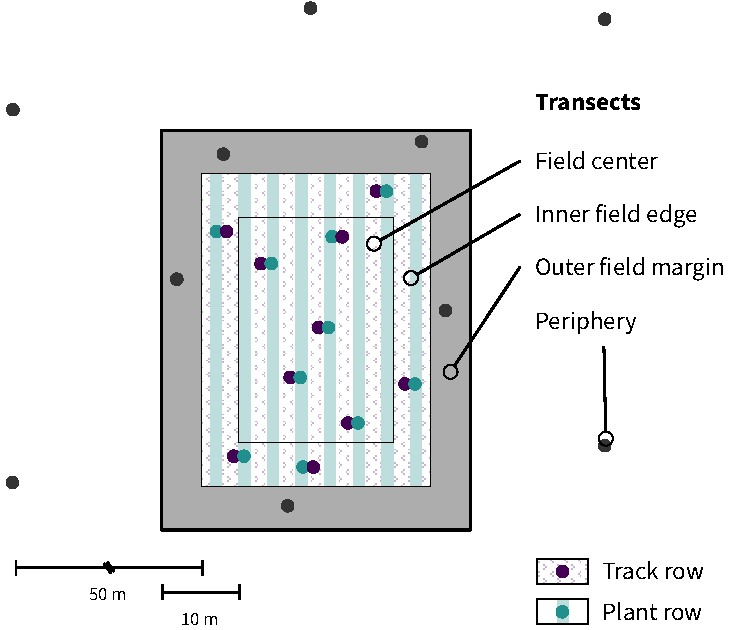
\includegraphics[width=3.267in]{figures/transects}
	\caption[Sampling scheme.]{Sampling scheme for one exemplary site; soil samples (filled dots, $n = 5$ per transect) were randomly selected. At the cultivated field centers and inner field edges, plant and track rows were sampled separately. The outer field margin and the field periphery were uncultivated.}
	\label{fig:transects}
\end{figure}

\subsection{Soil Characterization and Chemical Analysis of Plastic Covers}
\label{subsec:characterization}

The soil texture on each site was estimated from composite subsamples using the hydrometer method described in \citet{ASTMD422-63Standard2007}. The \ac{ec} and pH were measured in deionized water and \SI{0.01}{\Molar} \ch{CaCl_2} aqueous solution, respectively. Soil \ch{C} and \ch{N} were determined by dry combustion elemental analysis\sidenote{Vario MICRO Cube, Elementar, Germany.}.

The grab-sampled plastic covers were characterized by qualitative \ac{ted-gc-ms} and \ac{py-gc-ms}, \ac{dsc}, \ac{tga}, and \ac{ftir}--\ac{atr} analysis.
\ac{ted-gc-ms} and \ac{py-gc-ms} were applied to assess volatile additives or other polymer\-/associated compounds as well as the overall polymer composition of the agricultural plastic covers. To this end, a \num{1}\,\texttimes\,\SI{1}{\square\milli\meter} piece was cut out of each plastic cover and placed into a pyrolyzer quartz tube of a Pyroprobe 6150 filament pyrolyzer\sidenote{CDS Analytical, Oxford, US.} coupled with a Trace GC Ultra with DSQII \ac{ms}\sidenote{Thermo Fisher Scientific, Bremen, Germany.}.
For the \ac{ted-gc-ms} analysis, the pyrolyzer interface was flash heated (\SI{10}{\kelvin\per\milli\second}) to \SI{300}{\degreeCelsius} for \SI{15}{\second} to volatilize any polymer\-/associated compounds. A passivated transfer line (\SI{350}{\degreeCelsius}) transferred the volatiles to the \ac{ssl} injector (\SI{300}{\degreeCelsius}, split ratio 1:75) of the \ac{gc-ms} system.
The compounds were chromatographically separated in a \SI{1.3}{\milli\liter\per\minute} \ch{He} flow on a \SI{30}{\meter}\,\texttimes\,\SI{0.25}{\milli\meter} capillary column (\SI{5}{\percent} phenyl-arylene, \SI{95}{\percent} dimethylpolysiloxane, \SI{0.25}{\micro\meter} film thickness)\sidenote{ZB-5MS, Phenomenex, Aschaffenburg, Germany.}. The oven program was: \SI{40}{\degreeCelsius} (\SI{2}{\minute} hold), \SI{8}{\kelvin\per\minute} ramp to \SI{300}{\degreeCelsius} (\SI{5}{\minute} hold). The \ac{gc-ms} transfer line was kept at \SI{280}{\degreeCelsius}, and the \ac{ms} ion source (\SI{70}{\electronvolt}) was heated to \SI{230}{\degreeCelsius}. The \ac{ms} monitored \SIrange{50}{280}{\mz} at a scan rate of \SI{500}{\per\second}.
After \ac{ted-gc-ms}, the sample was pyrolyzed at \SI{750}{\degreeCelsius} for \SI{15}{\second} applying the same \ac{gc-ms} settings. All chromatograms were evaluated using OpenChrom, version 1.4.0.202103172155 \citep{WenigOpenChrom2010}, with the NIST08 database for peak identification.

\ac{dsc} and \ac{tga} measurements were conducted in accordance with Chapter~\ref{ch:tga-ms-method}. In brief, \ac{dsc} was applied between \SIrange[range-phrase={ and }]{-50}{250}{\degreeCelsius} (\SI{10}{\kelvin\per\minute} ramp, \SI{50}{\milli\liter\per\minute} \ch{N_2} flow)\sidenote{Q1000, TA Instruments, New Castle, US.} to determine the melting and crystallization temperatures of the agricultural plastic films.
For the determination of polymer degradation onsets and evolved gases, plastic samples were subjected to \ac{tga}\sidenote{STA 449 F3 Jupiter with QMS 403 C Aëolos, Netzsch, Selb, Germany.}. The heating ramp was \SI{5}{\kelvin\per\minute} from \SIrange[range-phrase={ to }]{40}{1000}{\degreeCelsius} under a \SI{20}{\milli\liter\per\minute} \ch{Ar} flow. The degradation onset was determined by the temperature at which the polymer starts to thermally decompose (\SI{<1}{\percent} mass loss).

Complementary \ac{ftir}--\ac{atr} analyses were performed between \SIrange[range-phrase={ and }]{4000}{650}{\per\centi\meter} at a resolution of \SI{4}{\per\centi\meter} using a Cary 630 spectrometer\sidenote{Agilent, Santa Clara, California, US.}. Peaks were identified with Open Specy, version 0.9.2 \citep{CowgerMicroplastic2021}.

\subsection{Soil Sample Preparation and Visual Pre-screening}
\label{sec:sample-prep}

All soil cores were sieved to fine soil (\SI{<=2}{\milli\meter}) and manually homogenized as suggested in Chapter~\ref{ch:analytical-techniques}. Visual plastic items retained by the sieve (\SI{>2}{\milli\meter}) were picked, photographed\sidenote{Leica S9i, Wetzlar, Germany.}, and analyzed via \ac{ftir}--\ac{atr} as described in the previous section.

Plastic debris \SI{<=2}{\milli\meter} were density-separated from the soil matrix using saturated \ch{NaCl} solution. To this end, \SI{50}{\gram} of fine soil were first weighted into \SI{1}{\liter} separation funnels with \ac{ptfe} stop cock\sidenote{Carl Roth, Karlsruhe, Germany.} and agitated at \SI{150}{rpm} with \SI{125}{\milli\liter} of sodium hexametaphosphate\sidenote{\cas{68915-31-1}, \SI{>=99}{\percent} purity, Carl Roth, Karlsruhe, Germany.} solution (\SI{40}{\gram\per\liter}) for \SI{2}{\hour} to disperse any soil aggregates. In a second step, \SI{90}{\gram} of \ch{NaCl}\sidenote{\cas{7647-14-5}, \SI{>=99.8}{\percent} purity, Carl Roth, Karlsruhe, Germany.} and \SI{125}{\milli\liter} of ultra-pure water were added to obtain a density solution of \SI{1.2}{\gram\per\cubic\centi\meter}. The mixture was shaken for another \SI{2}{\hour} and left for sedimentation for at least \SI{16}{\hour}. The sedimented soil was released from the separation funnel by gentle stirring of the suspension using the curved end of a bicycle spoke. Afterwards, the supernatant was collected in pleated cellulose filters with a particle retention of \SIrange{4}{12}{\micro\meter}\sidenote{Whatman 589/2, GE Healthcare, Buckinghamshire, UK.}. The filter cakes were transferred into glass culture tubes \sidenote{\num{16}\,\texttimes\,\SI{100}{\square\milli\meter}, GL18, VWR, Darmstadt Germany.} and dried at \SI{60}{\degreeCelsius}.

Based on Chapter~\ref{ch:py-gc-ms-method}, the culture tubes were topped off with \SI{8}{\milli\liter} of a 1:1-mixture (v+v) of \textit{p}-xylene\sidenote{\cas{106-42-3}, \SI{>98}{\percent} purity, Fluka Analytical, München, Germany.} and \ac{tcb}\sidenote{\cas{120-82-1}, \SI{99}{\percent} purity, Alfa Aesar, Kandel, Germany.}. In addition, the mixture contained \SI{100}{\milli\gram\per\liter} butylated hydroxytoluene\sidenote{\cas{128-37-0}, \SI{>=99}{\percent}, Merck, Darmstadt, Germany.} to prevent polymer oxidation.
The tubes were sealed with a \ac{ptfe} packing\sidenote{Carl Roth, Karlsruhe, Germany.}, vortexed, and heated at \SI{150}{\degreeCelsius} for \SI{1}{\hour} to facilitate the extraction of the polymer analytes from the filter cake.
After cooling down to room temperature, the supernatant was spiked with deuterated \ac{ps} (\ac{ps}-d5)\sidenote{PolymerSource, Quebec, Canada.} for internal standardization using positive displacement pipettes with glass capillaries\sidenote{Transferpettor micro, Brand, Wertheim, Germany.}. The extracts were stored in \SI{2}{\milli\liter} ND9 glass vials with inserts and \ac{ptfe}-sealed caps\sidenote{Wicom, Heppenheim, Germany.}.

\subsection{Quantification of Plastic Debris in Soil}

\ac{pe}, \ac{pp}, and \ac{ps} debris in fine soil (\SI{<=2}{\milli\meter}) were quantified via \ac{py-gc-ms} as detailed in Chapter~\ref{ch:py-gc-ms-method}.
In brief, \SI{2}{\micro\liter} sample aliquots were injected into pyrolyzer quartz tubes equipped with two microfiber filter discs\sidenote{Whatman QM-A, Kent, UK.} using a \SI{10}{\micro\liter} syringe with \ac{ptfe} plunger\sidenote{Hamilton 1701 N with 26s gauge, Bonaduz, Switzerland.}.
Each sample was measured once as described in Section~\ref{subsec:characterization}. However, the pyrolyzer interface was first held at \SI{300}{\degreeCelsius} to purge remaining solvents and volatiles on-line. After \SI{3}{\minute}, the sample was flash pyrolyzed (\SI{10}{\kelvin\per\milli\second}) at \SI{700}{\degreeCelsius} for \SI{15}{\second} and transferred to the \ac{gc-ms} system. The \ac{ms} selectively monitored \SIlist{70;126}{\mz} for the \ac{pp} pyrolysate 2,4-dimethyl-1-heptene (2,4Me9:1(1), \ac{ri} \num{841}), \SIlist{104;118}{\mz} for the \ac{ps} pyrolysates styrene (Sty, \ac{ri} \num{895}) and $\alpha$-methylstyrene ($\alpha$MeSty, \ac{ri} \num{981}), respectively, and \SIlist{82;95}{\mz} for \ac{pe} \textit{n}-alkadienes like 1,21-docosadiene (22:2(1,21), \ac{ri} \num{2187}). The internal standard styrene-d5 (Sty-d5, \ac{ri} \num{892}) was acquired at \SI{109}{\mz}.

\subsection{Method Validation}

The reference polymers used for external standardization and recovery experiments were analytical grade \ac{pe} beads\sidenote{\cas{9002-88-4}, \SI{500}{\micro\meter} average particle size, Alfa Aesar, Kandel, Germany.}, \ac{pp} fragments\sidenote{\cas{9003-07-0}, isotactic, \SI{<=1000}{\micro\meter}, Aldrich Chemistry, Taufkirchen, Germany.}, and \ac{ps} beads\sidenote{\cas{9003-53-6}, \SI{250}{\micro\meter} average particle size, Goodfellow, Huntingdon, UK.} (see Chapter~\ref{ch:py-gc-ms-method} for details).

The \ac{py-gc-ms} system was calibrated weekly against external standards (\SIrange{5}{200}{\micro\gram\per\milli\liter} \ac{pe}, \ac{pp}, and \ac{ps} dissolved in \textit{p}-xylene/\ac{tcb} at \SI{150}{\degreeCelsius}) following the protocol outlined in Chapter~\ref{ch:py-gc-ms-method}. Calibration curves were evaluated for signal sensitivity (slope) and linearity (adj. $R^2$). Daily sample measurements were bracketed with \SI{100}{\micro\gram\per\milli\liter} standards to correct for inter-day variations. The intra-day repeatability was determined by consecutive injections of \SI{100}{\micro\gram\per\milli\liter} standards ($n$ = 12). The internal standard \ac{ps}-d5 added after sample extraction was used for continuous repeatability checks of sample measurements.

To evaluate the plastic recovery from soil, triplicates of two agricultural reference soils were spiked at \SIlist{2;20}{\milli\gram\per\kilo\gram} of each polymer. The used reference soils were a loamy sand (\SI{8}{\percent} clay, \SI{16}{\percent} silt, \SI{76}{\percent} sand) with a \ch{C_{org}} content of \SI{1.7}{\percent} (LUFA 2.2) \sidenote{\foreignlanguage{ngerman}{Landwirtschaftliche Untersuchungs- und Forschungsanstalt, Speyer}, Germany.} and a silty clay (\SI{47}{\percent} clay, \SI{41}{\percent} silt, \SI{12}{\percent} sand) with \SI{2.5}{\percent} \ch{C_{org}} (RefeSol 06-A)\sidenote{Fraunhofer IME, Schmallenberg, Germany.}.
Instrumental and method \acp{lod} and \acp{loq} were calculated from standard deviations (\ac{sd}s) of signal intensities of low analyte concentrations (\SI{2}{\micro\gram\per\milli\liter}) and blank reference soils ($n$ = 3), respectively, in accordance with Chapter~\ref{ch:py-gc-ms-method}, \citet{DIN32645Chemical2008}, and \citet{MagnussonEurachem2014}. The selectivity against other potentially interfering non-target polymers was estimated from peak intensities of \ac{pe}, \ac{pp}, and \ac{ps} pyrolysates in LUFA 2.2 soil spiked at each \SI{40}{\milli\gram\per\kilo\gram} \ac{pet}, \ac{pmma}, \ac{pvc}, and \ac{twp}. The \ac{pet} came from a cryomilled bottle recyclate\sidenote{PETKA CZ, Brno, Czech Republic.} as detailed in Chapter~\ref{ch:tga-ms-method}. The \ac{pmma} was ground from a commercial plexiglass\sidenote{\foreignlanguage{ngerman}{Bundesanstalt für Materialforschung und -prüfung}, Berlin, Germany.}. The \ac{pvc} was purchased from Aldrich Chemistry\sidenote{Taufkirchen, Germany.}, and the \ac{twp} was from a test rig at \foreignlanguage{ngerman}{Bundesanstalt für Straßenwesen}\sidenote{Bergisch Gladbach, Germany.}.
In addition, a matrix-matched calibration was performed in LUFA 2.2 soil extracts in accordance with \citet{MagnussonEurachem2014} to assess the effect of soil matrix on the calibration parameters.

\subsection{Quality Control}

To prevent the risk of contamination, all laboratory equipment coming into direct contact with the sample or the extract solution was made of glass, metal, paper, or \ac{ptfe}. \ac{pe}, \ac{pp}, or \ac{ps} equipment was completely avoided. The worn laboratory coats were of \SI{100}{\percent} cotton. In addition, all samples and extracts were kept in closed vessels or covered with aluminum foil. The vessels were only opened under a fume hood.

The sample extraction was monitored with weekly procedural blanks that underwent the complete extraction procedure as the samples but without soil addition. Plastic contents in our procedural blanks were exclusively below the \ac{lod}.

\subsection{Data Evaluation}

Data processing and statistical analyses were conducted using R (version 4.1.0) with ``data.table'', ``magrittr'', and ``envalysis'' as main libraries. The results are given as
mean\,\textpm\,\ac{sd}. Measurement repeatabilities are stated as percentage \ac{rsd}. Matches from the Open Specy \ac{ftir} library are reported as Pearson's $r$.

The potential matrix effect on the calibration was evaluated using \ac{sse} ratios (Eq.~\ref{eq:sse}) which compare
the slope of a calibration curve prepared in solvent ($b_\mathrm{solv}$) with that of the matrix-matched calibration
($b_\mathrm{matrix}$) \citep{MagnussonEurachem2014}.

\begin{equation}
	\label{eq:sse}
	\mathrm{\ac{sse}} = \frac{b_\mathrm{matrix} - b_\mathrm{solv}}{b_\mathrm{solv}}
\end{equation}

\section{Results and Discussion}

\subsection{Soil Properties}

According to \citet{FAOWorld2014} classification, the investigated soils were identified as anthrosols. The dominant soil textures were silty clay and clayey silt (Table~\ref{tab:soils}), with sites 1, 3, and 4 showing the highest clay contents (\SI{>30}{\percent}) compared to the remaining sites. Sites 1--3 and sites 6--7 had \ch{C_{org}} contents of \SIrange{1.1}{1.3}{\percent} and \SIrange{1.4}{1.5}{\percent}, respectively. The lowest \ac{Corg} contents (\SI{0.9}{\percent}) were found on sites 4 and 5. Soil \ch{N} was \SI{<=0.2}{\percent} across all sites. The soil pH was slighly acidic (\numrange{6.6}{7.0}), and the \ac{ec} ranged from \SIrange[range-phrase={ to }]{118}{536}{\micro\siemens\per\centi\meter}. The highest \ac{ec} values were observed on sites 6 and 7.

\begin{table*}
	\centering\footnotesize
	\caption{Soil properties of experimental sites.}\label{tab:soils}
	\begin{tabular}{lllS[table-format = 2]S[table-format = 2]S[table-format = 2]lS[table-format = 1.1]S[table-format = 1.1]S[table-format = 1.1]S[table-format = 1.1]S[table-format = 3]}
		\toprule
		{Site} & {Cover (bottom to top)} & {Location} & {Clay} & {Silt} & {Sand} & {Texture\textsuperscript{\textdaggerdbl}} & {\ch{C_{org}}} & {\ch{C_{total}}} & {\ch{N_{total}}} & {pH} & {\ac{ec}} \\
		& & & {[\si{\percent}]} & {[\si{\percent}]} & {[\si{\percent}]} & & {[\si{\percent}]} & {[\si{\percent}]} & {[\si{\percent}]} &  & {[\si{\micro\siemens\per\centi\meter}]} \\
		\midrule
		1 & Fleece (\ac{pp}), perforated foil (\ac{pe}) & Offenbach & 34 & 53 & 13 & Tu3 & 1.3 & 1.3 & 0.1 & 6.6 & 200 \\
		2 & Mulch (\ac{pe}), fleece (\ac{pp}) & Offenbach & 10 & 77 & 13 & Ut2 & 1.1 & 1.3 & 0.1 & 6.8 & 138 \\
		3 & Mulch (\ac{pe}) & Offenbach & 36 & 64 & 0 & Tu3 & 1.2 & 1.4 & 0.1 & 6.8 & 147 \\
		4 & Fleece (\ac{pe}), perforated foil (\ac{pe}) & Schifferstadt & 32 & 67 & 1 & Tu4 & 0.9 & 1.1 & 0.1 & 6.7 & 118 \\
		5 & Fleece (\ac{pe}), perforated foil (\ac{pe}) & Schifferstadt & 24 & 76 & 0 & Ut4 & 0.9 & 1.1 & 0.1 & 6.9 & 236 \\
		6 & Perforated foil (\ac{pe}) & Landau & 25 & 75 & 0 & Ut4 & 1.4 & 1.6 & 0.2 & 6.8 & 510 \\
		7 & Perforated foil (\ac{pe}) & Landau & 21 & 79 & 0 & Ut4 & 1.5 & 1.6 & 0.2 & 6.9 & 536 \\
		8 & Perforated foil (\ac{pe}) & Landau & 15 & 85 & 0 & Ut3 & 1.4 & 1.6 & 0.2 & 7.0 & 289 \\
		\bottomrule
		\multicolumn{12}{p{.9\textwidth}}{\textsuperscript{\textdaggerdbl} In accordance with \citet{SponagelBodenkundliche2005}; Tu = silty clay, Ut = clayey silt.} \\~
	\end{tabular}
\end{table*}

\subsection{Agricultural Plastic Covers}

The fleeces that covered sites 1 and 2 were identified as \ac{pp} as indicated by multiple \ch{C-H} stretch deformations at \SIrange{2950}{2838}{\per\centi\meter} as well as \ch{CH_2} and \ch{CH_3} bends at \SIlist{1455;1377}{\per\centi\meter}, respectively (Open Specy \ac{ftir} library match: $r \geq$ \num{0.96}, see Figure~\ref{fig:ftir-covers}a for an exemplary \ac{ftir} spectrum). A shapeless broad peak between \SIrange[range-phrase={ and }]{1860}{1660}{\per\centi\meter} indicated the presence of carbonyl groups \citep{GrauseChanges2020}. The indistinct band between \SIrange[range-phrase={ and }]{1200}{900}{\per\centi\meter} may be attributed to \ch{C-O} stretching in alcohols, acids, or ethers originating from a contamination with \ac{som} or plastic aging \citep{FuMechanism2021}. Complementary \ac{dsc} showed crystallization temperatures at \SIlist{114;116}{\degreeCelsius} and melting temperatures at \SIlist{158;160}{\degreeCelsius}. Between \SIrange[range-phrase={ and }]{381}{400}{\degreeCelsius}, the polymers started to decompose into methylalkenes characteristic for \ac{pp} \citep[Figure~\ref{fig:py-covers}a for an exemplary pyrogram]{TsugePyrolysis2011}.

By contrast, the fleece from sites 4 and 5 was made of \ac{pe} ($r$ = \num{0.96}). The respective \ac{ftir} spectrum showed indicative \ch{CH_2} stretching between \SIrange{2919}{2915}{\per\centi\meter} (asymmetric)
and \SIrange{2851}{2845}{\per\centi\meter} (symmetric, Figure~\ref{fig:ftir-covers}c). The crystallization and melting temperatures were \SIlist{96;108}{\degreeCelsius}, respectively. The degradation onset was \SI{408}{\degreeCelsius} and triggered the formation of \ac{pe}-specific triplets of $n$-alkadienes, $n$-alkenes, and $n$-alkanes (Figure~\ref{fig:py-covers}c).
All other covers, namely mulches and perforated foils from sites 2--8, were made of \ac{pe} ($r \geq$ 0.86, Figure~\ref{fig:ftir-covers}b,d,e). The carbonyl band at \SIrange{1860}{1660}{\per\centi\meter} was visible in all samples but was most pronounced for the \ac{pe} mulch from sites 2 and 3. However, crystallization temperatures (\SIrange{100}{113}{\degreeCelsius}) and melting temperatures (\SIrange{110}{122}{\degreeCelsius}) of the \ac{pe} mulch were slightly higher than those of the \ac{pe} fleece. The degradation onsets of the mulches and perforated foils ranged from \SIrange[range-phrase={ to }]{384}{397}{\degreeCelsius}.

The qualitative analyses of volatile polymer additives and other polymer\-/associated compounds thermally desorbing from the agricultural films at \SI{300}{\degreeCelsius} revealed three omnipresent substances (NIST08 matches \SI{>75}{\percent}, see Figure~\ref{fig:ms-covers}): These were propyl dodecanoate\sidenote{\cas{3681-78-5} or \cas{10233-13-3}.}, oleonitrile\sidenote{\cas{112-91-4}.}, and 9-octadecenamide\sidenote{\cas{301-02-0}.} (see Figure~\ref{fig:py-covers} for exemplary chromatograms). In addition, the \ac{pp} fleeces from sites 1 and 2 as well as the \ac{pe} perforated foils from sites 4--8 contained traces of a di-\textit{tert}-butylphenol\sidenote{For instance \cas{96-79-4}.} which is an indicator for antioxidants \citep{HahladakisOverview2018}. Propyl dodecanoate and oleonitrile are lubricants probably added to agricultural plastic covers for easier spreading out on site. 9-Octadecenamide is a known degradation product of hindered amine light stabilizers like Chimassorb 944 \citep{HaiderLoss2001}. No pesticides were detected in the plastic covers, probably due to the limited sensitivity of the qualitative analysis and/or their low thermal stability.

Complementary \ac{ftir}--\ac{atr} and \ac{py-gc-ms} confirmed that both plastic mulches and perforated foils were exclusively made of \ac{pe}. The fleeces were of \ac{pe} and \ac{pp}, although \ac{pp} is more common \citep{HamouzInfluence2011}. All \ac{pe} covers melted within the range of \SIrange{109}{125}{\degreeCelsius} and degraded \SI{>318}{\degreeCelsius} as expected for virgin low-density \ac{pe} \citep{BeylerThermal2002}. Interestingly though, melting temperatures of the \ac{pp} fleeces were \SIrange[range-phrase={ to }]{5}{10}{\degreeCelsius} lower than those of virgin \ac{pp} (\SIrange{165}{170}{\degreeCelsius}) \citep{BeylerThermal2002,TochacekPolymer2019}. The degradation onset was not affected by this and comparable to virgin \ac{pp} (\SI{>315}{\degreeCelsius}) \citep{BeylerThermal2002}. Decreasing melting temperatures may indicate the presence of additives or other impurities but could also be a first sign of polymer aging as similarly observed after \numrange{5}{20} months of temperate weathering \citep{TochacekPolymer2019}. This is consistent with the carbonyl groups identified via \ac{ftir} which are indicative for the photo-oxidation of polyolefins \citep{GrauseChanges2020}. In our study, fleeces and perforated foils were on the fields for about four months. The mulches were applied two years previously. The incipient aging concurred with the release of antioxidant di-\textit{tert}-butylphenol from the \ac{pp} backbone as indicated by \ac{ted-gc-ms}. As di-\textit{tert}-butylphenol was also released from \ac{pe} perforated foils, it remains unresolved whether the presence of di-\textit{tert}-butylphenol was material-specific or indeed triggered by polymer aging.

\subsection{Visual Plastic Items on Site}

We visually identified 30 suspect items (\SI{>2}{\milli\meter}) during soil sieving. Subsequent \ac{ftir}--\ac{atr} analysis revealed six items as plastics. These were a black \ac{pe} film ($r$ = 0.92, Figure~\ref{fig:visual-items}a) and four \ac{ps} fragments ($r \geq$ 0.91, Figure~\ref{fig:visual-items}b) at the field center of site 5 (see Figure~\ref{fig:ftir-debris} for the respective \ac{ftir} spectra). The \ac{ps} showed characteristic peaks at \SIlist{3024;1492;694}{\per\centi\meter} originating from aromatic \ch{C-H} stretch and bend deformations. In the field center of site 6, a green \ac{pe} film ($r$ = 0.92, Figure~\ref{fig:visual-items}c) was found. All other items were of natural origin including invertebrate shells, stones or wood fragments, and cellulose fibers that were identified by Open Specy as chitin, resin dispersion, and cotton, respectively ($r \geq$ 0.82, Figure~\ref{fig:visual-items}d--f).

\begin{figure*}
	\centering
	\includegraphics[width=12cm]{figures/visual-items}
	\caption[Exemplary photographs of suspect particles \SI{>2}{\milli\meter}.]{(a) \ac{pe} film and (b) \ac{ps} fragment from the field center of site 5, (c) \ac{pe} film and (d) chitin shell from the field center of site 6, and (e) resin or natural fragment and (f) cotton fiber from the field edge of site 7; see Figure~\protect\ref{fig:ftir-debris} for the respective \ac{ftir} spectra.}
	\label{fig:visual-items}
\end{figure*}

In this respect, it is important to note that the visual identification of suspect items largely depends on the operator's experience and may thus lead to excessive over- or underestimation of particle numbers (Chapter~\ref{ch:analytical-techniques}). Furthermore, counting suspect items \SI{>2}{\milli\meter} in a \SI{100}{\cubic\centi\meter} soil core is hardly representative. We thus refrained from extrapolating our findings to particles\,\si{\per\kilo\gram} and intended visual identification to serve as a qualitative complement to subsequent \ac{py-gc-ms} quantification.
Interestingly though, the plastic debris \SI{>2}{\milli\meter} were exclusively found on sites 5 and 6. None of the black and green \ac{pe} or white \ac{ps} fragments matched the applied white \ac{pe} fleece and perforated foil in color or polymer type. This suggests an external source of plastic debris, for instance from adjacent streets or other fields, or residues from previous land use \citep{HarmsAmount2021}.

\subsection{\ac{py-gc-ms} Method Performance}

The pyrolysates chosen for quantifying \ac{pe}, \ac{pp}, and \ac{ps} were 22:2(1,21), 2,4Me9:1(1), and Sty, respectively, as they performed the best in terms of signal linearity (adj. $R^2 >$ \num{0.995}), instrumental \acp{lod} (\SI{<10}{\nano\gram}), and measurement repeatability (\ac{rsd} \SI{<10}{\percent}, Table~\ref{tab:py-instrument}). The $n$-alkadiene 22:2(1,21) was preferred over the respective $n$-alkene or $n$-alkane because of its higher selectivity for \ac{pe} (Chapter~\ref{ch:py-gc-ms-method}). LUFA 2.2 exerted a negligible matrix effect of \SIlist{16;-3;-2}{\percent} \ac{sse} on the selected \ac{pe}, \ac{pp}, and \ac{ps} pyrolysates (see Figure~\ref{fig:matrix-match} for calibration curves). Method \acp{lod} were \SIrange{0.7}{1.2}{\milli\gram\per\kilo\gram} in RefeSol 06-A and \SIrange{1.9}{3.3}{\milli\gram\per\kilo\gram} in LUFA 2.2. The respective method \acp{loq} ranged from \SIrange[range-phrase={ to }]{2.5}{9.5}{\milli\gram\per\kilo\gram} (Table~\ref{tab:py-validation}). A LUFA 2.2 soil containing each \SI{40}{\milli\gram\per\kilo\gram} of potentially interfering, non-target \ac{pet}, \ac{pmma}, \ac{pvc}, and \ac{twp} did not induce significant false positive detections of \ac{pe}, \ac{pp}, or \ac{ps}.

\begin{table}
	\centering\footnotesize
	\caption{Instrumental validity criteria of the \ac{py-gc-ms} method.}\label{tab:py-instrument}
	\begin{tabular}{llS[table-format = 1.4]S[table-format = 2.1]S[table-format = 2.1]}
		\toprule
		{Polymer} & {Pyrolysate} & {adj. $R^2$} & {\ac{lod}\textsuperscript{\textasteriskcentered}} & {\ac{rsd}} \\
		& & & {[\si{\nano\gram}]} & {[\si{\percent}]} \\
		\midrule
		\ac{pe} & 17:2(1,16) & 0.9912 & 9.0 & 11.3 \\
		& 18:2(1,17) & 0.9785 & 9.2 & 9.8 \\
		& 19:2(1,18) & 0.9965 & 5.6 & 11.3 \\
		& 20:2(1,19) & 0.9788 & 6.4 & 11.9 \\
		& 21:2(1,20) & 0.9897 & 10.0 & 12.8 \\
		& 22:2(1,21) & 0.9952 & 5.8 & 9.5 \\
		& 23:2(1,22) & 0.9709 & 7.2 & 11.2 \\
		\ac{pp} & 2,4Me9:1(1) & 0.9997 & 4.6 & 8.9 \\
		\ac{ps} & Sty & 0.9980 & 6.6 & 3.5 \\
		& $\alpha$MeSty & 0.9866 & 19.4 & 11.5 \\
		\bottomrule
		\multicolumn{5}{p{.55\textwidth}}{\textsuperscript{\textasteriskcentered} Instrumental limit of detection; \ac{rsd} = relative standard deviation.}
	\end{tabular}
\end{table}

\begin{table*}
	\centering\footnotesize
	\caption{Validation criteria of the extraction method.}\label{tab:py-validation}
	\begin{tabular}{llS[table-format = 1.1]S[table-format = 1.1]S[table-format = 1.1(1)]S[table-format = 3(2)]S[table-format = 3(2)]}
		\toprule
		{Polymer} & {Pyrolysate} & {\ac{lod}\textsuperscript{\textasteriskcentered}} & {\ac{loq}\textsuperscript{\textasteriskcentered}} & {Interference\textsuperscript{\textdagger}} & \multicolumn{2}{c}{Recovery} \\
		\cmidrule(lr){6-7}
		& & {[\si{\milli\gram\per\kilo\gram}]} & {[\si{\milli\gram\per\kilo\gram}]} & {[\si{\milli\gram\per\kilo\gram}]} & {at \SI{2}{\milli\gram\per\kilo\gram} [\si{\percent}]} & {at \SI{20}{\milli\gram\per\kilo\gram} [\si{\percent}]}\\
		\midrule
		\multicolumn{6}{l}{\textit{LUFA 2.2}} \\
		\ac{pe} & 22:2(1,21) & 1.9 & 9.5 &  0.9(3) & 133(9) & 105(3) \\
		\ac{pp} & 2,4Me9:1(1) & 2.9 & 2.9 & 0(0) & 70(10) & 93(5) \\
		\ac{ps} & Sty & 3.3 & 6.2 & 0(0) & 52(2) & 86(4) \\
		\multicolumn{6}{l}{\textit{RefeSoil 06-A}} \\
		\ac{pe} & 22:2(1,21) & 1.2 & 9.5 & & 30(20) & 50(10) \\
		\ac{pp} & 2,4Me9:1(1) & 0.8 & 2.5 & & 30(20) & 62(1) \\
		\ac{ps} & Sty & 0.7 & 6.2 & & 0(0) & 12(5) \\
		\bottomrule
		\multicolumn{7}{l}{\textsuperscript{\textasteriskcentered} Method limits of detection and quantification; \textsuperscript{\textdagger} introduced from \SI{40}{\milli\gram\per\kilo\gram} non-target polymers.} \\~
	\end{tabular}
\end{table*}

The extraction of \SI{20}{\milli\gram\per\kilo\gram} plastic debris from LUFA 2.2 soil yielded recoveries of \SIrange{86}{105}{\percent} (Table~\ref{tab:py-validation}). \ac{pe} was recovered the best whereas \ac{ps} showed the lowest value. Recovering plastic debris at levels close to the method \ac{lod} (\SI{2}{\milli\gram\per\kilo\gram}) and below the respective method \acp{loq} led to an overestimation of recovered \ac{pe} (\SI{133(9)}{\percent}) while underestimating \ac{pp} (\SI{70}{\percent}) and \ac{ps} (\SI{50}{\percent}). Recoveries from RefeSol 06-A were generally lower: Whereas we still recovered \SIlist{50;62}{\percent} of the \SI{20}{\milli\gram\per\kilo\gram} \ac{pe} and \ac{pp}, respectively, recoveries dropped to \SI{30(20)}{\percent} at the lower spiking level. Hardly any \ac{ps} was recovered from RefeSol 06-A (\SI{<12}{\percent}) irrespective of the spiking level.

As reviewed in Chapter~\ref{ch:analytical-techniques}, several studies have already evaluated their extraction procedures for various plastic debris from solid matrices using organic solvents like \ac{dcm} or \ac{thf}. In combination with quantitative \ac{py-gc-ms}, however, matrix interferences and false positive detections from organic matrix constituents or other non-target polymers should be closely monitored (\citealp{DierkesQuantification2019}; Chapter~\ref{ch:py-gc-ms-method}).
By combining density separation and solvent extraction with \textit{p}-xylene/\ac{tcb}, we obtained method \acp{lod} from blank LUFA 2.2 and RefeSol 06-A and interferences from non-target polymers equivalent \SI{<3.3}{\milli\gram\per\kilo\gram} \ac{pe}, \ac{pp}, and \ac{ps}, which highlights the selectivity of our method. Dispersing soil aggregates with sodium hexametaphosphate prior to density separation further enabled the quantification of plastic debris potentially occluded in or masked by soil aggregates. The required filtration step, however, systematically excluded particles \SI{<4}{\micro\meter} that were not retained by the applied filter.

Inconsistent recoveries at a spiking level below the method \acp{loq} of \SIrange[range-phrase={ to }]{2.5}{9.5}{\milli\gram\per\kilo\gram} challenged the sensitivity and robustness of our solvent-based approach. This particularly applied to the \SI{<30}{\percent} \ac{pe}, \ac{pp}, and \ac{ps} we recovered from RefeSol 06-A. While this clearly defines the quantitative limits of the method, our working range is still \numrange{10}{100} times lower than that of previous applications involving solvent-based \ac{py-gc-ms}. \Citet{DierkesQuantification2019,OkoffoIdentification2020}, for instance, spiked \SI{1}{\gram} of quartz sand and biosolids at \SIrange{0.05}{50}{\gram\per\kilo\gram} of various polymers to evaluate their accelerated solvent extraction with \ac{thf} and \ac{dcm}, respectively.
Irrespective of the spiking level though, our \ac{ps} recoveries from the clayey RefeSol 06-A were particularly low (\SI{<12}{\percent}). This is in line with \citet{WangPoor2018} who found comparable recoveries after density separation of nano-sized \ac{ps} from a silt soil. \citet{LuoDistribution2020,WuTransport2020} reasoned that \ac{som} as well as \ch{Fe} and \ch{Al} oxides effectively retain \ac{ps} particles in soil. The dramatic decrease in \ac{ps} recovery may be attributed to interactions forming between the delocalized $\pi$-electrons of the aromatic \ac{ps} ring and \ac{som}, iron and aluminum oxides, or cations bound to the negatively charged surface of clay particles \citep{NewcombDeveloping2017}. During the density separation, the aggregated \ac{ps} may have been preferentially sedimented, and thereby systematically excluded from subsequent solvent extraction. The addition of an anionic surfactant like sodium dodecyl sulfate or nonionic polysorbates during soil aggregate dispersion and density separation could counteract this, but potentially at the expense of introducing another source of \ac{pe} contamination from the surfactants' $n$-alkane domains.

Based on the two reference soils tested and on previous work (Chapter~\ref{ch:py-gc-ms-method}), we considered our method sufficiently sensitive and quantitative for environmentally-relevant \ac{pe} and \ac{pp} levels exceeding the respective method \acp{loq}. The \SI{50}{\percent} \ac{pe} and \SI{62}{\percent} \ac{pp} we recovered from RefeSol 06-A suggest a rather semi-quantitative evaluation of soils with a clay content \SI{>47}{\percent} and a \ch{C_{org}} content \SI{>2.5}{\percent}. \ac{ps} is evaluated qualitatively for its low recoveries.
These findings once more highlight the importance of specifically testing and evaluating analytical methods for plastic analysis with various soil types (Chapter~\ref{ch:analytical-techniques}). The extrapolation of specific validity criteria to field samples with a different texture and \ch{C_{org}} composition thus remains difficult and requires careful interpretation.

\subsection{\ac{pe}, \ac{pp}, and \ac{ps} Debris in Soil}

We detected plastic debris \SI{<=2}{\milli\meter} exceeding the average method \ac{lod} of \SIrange{1.5}{2.0}{\milli\gram\per\kilo\gram} in 15 out of 240 samples from six sites (Figure~\ref{fig:py-screening}). This is equivalent to \SI{6}{\percent} positive detections. Soil from sites 1, 7, and 8 contained the most \ac{pe} (10 findings) with single detections peaking at \SIlist{19;35}{\milli\gram\per\kilo\gram}. Mean \ac{pe} contents were the highest at the field margin of site 1 (\SI{10(10)}{\milli\gram\per\kilo\gram}) and decreased below the method \ac{lod} in the field edge and the field periphery. Furthermore, \ac{pe} contents were slightly higher in the track rows (furrows) than in the plant rows (ridges) of the field centers and edges of site 1. With \SIrange{4}{7}{\milli\gram\per\kilo\gram}, sites 7 and 8 showed maximum \ac{pe} contents in the field periphery. Field centers, edges, and margins contained less than \SI{2}{\milli\gram\per\kilo\gram} \ac{pe}. On these sites, differences in the \ac{pe} contents between field track and plant rows were mostly indistinct. Sites 2--6 did not contain any \ac{pe} above the method \ac{lod}.
The \ac{pp} findings were driven by single observations of \SIrange{5}{10}{\milli\gram\per\kilo\gram} in the field centers of sites 2, 4, and 7.
\ac{ps} was identified twice, namely in the periphery of sites 4 and 5. Due to the poor \ac{ps} recoveries, these findings are most likely underestimated.

\begin{figure*}
	\centering
	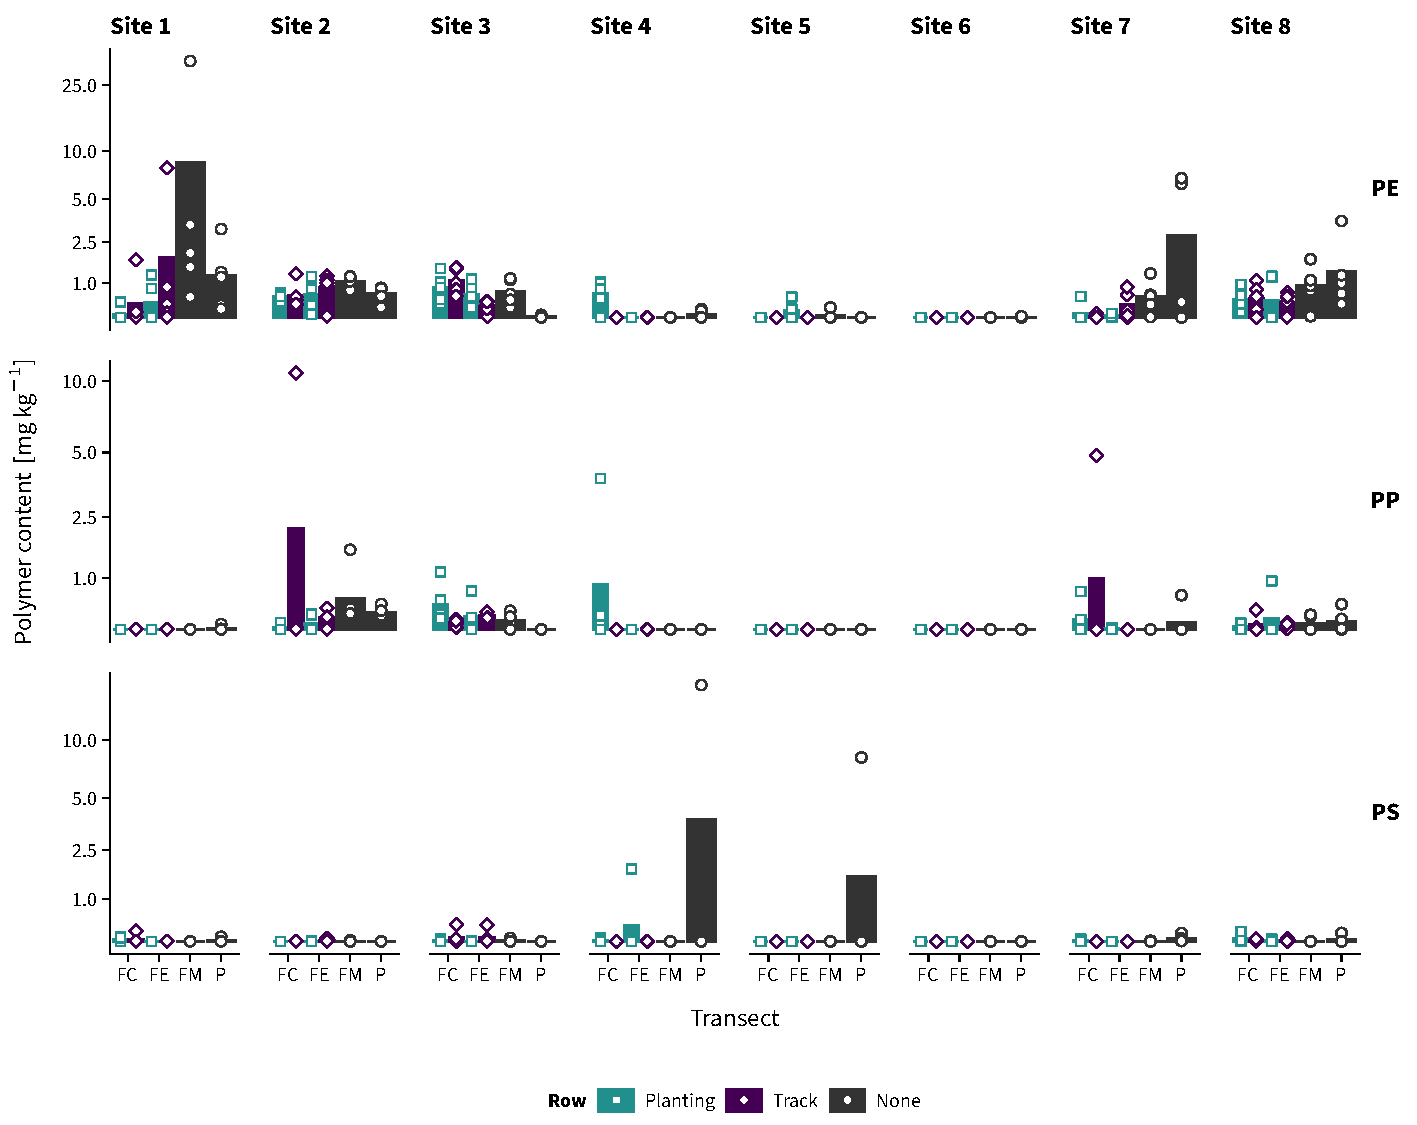
\includegraphics[width=\textwidth]{figures/py-screening}
	\caption[\Ac{pe}, \ac{pp}, and \ac{ps} contents (\SI{<=2}{\milli\meter}).]{Log-scaled \ac{pe}, \ac{pp}, and \ac{ps} contents (\SI{<=2}{\milli\meter}) at the field center (FC), field edge (FE), field margin (FM), and the periphery (P) of sites 1--8; dots represent single measurements, the underlying bar plot shows the transect average.}
	\label{fig:py-screening}
\end{figure*}

Interestingly, elevated \ac{pe} contents occurred mostly on sites 1, 7, and 8 which were covered with \SI{40}{\micro\meter} thick perforated foils. Sites 4--6 covered with thicker mulch films or perforated foils (\SI{50}{\micro\meter}) did not show any significant \ac{pe} contamination.
On the one hand, this is remarkable because the agricultural films were on site for four months only. On the other hand, the elevated plastic contents may have originated from another, potentially diffuse input source prior to plastic coverage.

Our results are yet in line with \citet{ZhangStatus2016} who attributed elevated plastic emissions to the use of particularly thin agricultural films. In China, for instance, common film thicknesses are \SIrange{6}{10}{\micro\meter}, while EU regulations stipulate agricultural covers thicker than \SI{20}{\micro\meter} \citep{EN13655Plastics2018}. This may also explain why studies conducted in non-EU countries often report extraordinarily high plastic levels in soil \citep{LiuWhite2014}, particularly after long-term use of agricultural plastics \citep{HuangAgricultural2020,ZhangDistribution2018}.

Regardless of the film thickness, the increased \ac{pe} contents at the field margin of site 1 suggested that the mechanical stress of weighing the plastic covers down with soil or digging them in favored the local formation of plastic debris. The close contact with soil and exposure to sunlight may have accelerated polymer aging and embrittlement as indicated by our complementary \ac{dsc} and \ac{ftir}--\ac{atr} measurements.
Due to the limited number of \ac{pe} detections above method \ac{lod}, we did not find a clear indication for the further translocation of plastic debris from the ridged plant rows to lower ground furrows. Tracing experiments by \citet{LaermannsTracing2021}, however, recently confirmed that the micro- and macrorelief of the soil surface may indeed favor the water erosion of plastic debris on a meter scale.
Even at larger scales though, it remained unresolved to what extent the \ac{pe} debris in the field periphery (mainly sites 7 and 8) originated from the covered field centers or whether it came from an external source via wind drift. Due to ubiquity of products made from \ac{pe}, such an external source cannot be excluded.

Although sites 1 and 2 were both fleeced with \ac{pp}, only site 2 showed elevated \ac{pp} contents. At the same time, \ac{pp} was found on sites covered exclusively with \ac{pe} for the last four months. Therefore, no clear association between \ac{pp} detections and the seasonal use of plastic covers was established. This is striking because the fibrous structure of the \ac{pp} fleece together with the initial signs of aging detected via \ac{dsc} and \ac{ftir}--\ac{atr} made emissions of plastic debris particularly likely.
Unexpectedly, these two study sites were thus most likely dominated by external sources like littering or previous land use rather than receiving plastic debris from the in situ fragmentation of fleeces.

This similarly applied to \ac{ps}, which is not used for agricultural plastic covers \citep{BertlingKunststoffe2021}, and may thus serve as an indicator for external sources of plastic debris in soil. Another possible explanation for the \ac{ps} findings on the two neighboring sites 4 and 5 may be a legacy contamination with \ac{ps}. In the past, beads made from expanded \ac{ps} were used for the conditioning and stabilization of horticultural soils \citep{MaghchicheUse2010}. However, it remained unresolved whether this was the case in the agricultural area investigated in this study.

Given that our investigated soils had a clay content of \SIrange{15}{36}{\percent}, the obtained \ac{pe}, \ac{pp}, and \ac{ps} contents were potentially
underestimated by a factor of \numrange{1.5}{2}. Even though taking this uncertainty into account, the plastic contents detected in our study were still up to \num{100} times lower than the \SI{820}{\milli\gram\per\kilo\gram} \ac{pe}, \SI{40}{\milli\gram\per\kilo\gram} \ac{pp}, and \SI{56}{\milli\gram\per\kilo\gram} \ac{ps} that \citet{DierkesQuantification2019} obtained from a non-characterized roadside soil using a comparable solvent-based \ac{py-gc-ms} method. A recent modeling study by \citet{BrandesIdentifying2021} estimated that plastic debris emitted from agricultural plastic covers may increase the plastic contents in agricultural soil by \SIrange{5}{9}{\milli\gram\per\kilo\gram} per year. By contrast, conversions from particle counts and shapes to plastic masses resulted in  contents of \SIrange{0.1}{1.2}{\milli\gram\per\kilo\gram} in agricultural soil covered with plastics \citep{BuksGlobal2020}. However, such conversions are increasingly discouraged for their high estimate errors \citep[Chapter~\ref{ch:analytical-techniques};][]{PrimpkeComparison2020}.
All this challenges comparisons since studies investigating plastic debris in agricultural soil so far exclusively used particle-based microspectroscropic techniques. Nonetheless, our results are approximately in the same order of magnitude than previous findings but should be further corroborated.

\section{Conclusions}

The combination of soil aggregate dispersion and density separation with solvent-based \ac{py-gc-ms} enabled the simple, yet selective quantification of \ac{pe} and \ac{pp} debris in agricultural soil. Analyzing a sample amount of \SI{50}{\gram} better accounted for the heterogeneous distribution of discrete plastic particles in the soil matrix. The additional dispersion step further made plastic debris occluded in soil aggregates amenable to quantification. By contrast, poor \ac{ps} recoveries potentially induced by that additional separation step challenged a reliable \ac{ps} quantification.

We applied the new method to soil randomly sampled from four predefined transects located in and around eight agricultural field covered with plastic films. This screening approach revealed first insights into the potential contribution of agricultural plastic covers to plastic pollution in soil: While \ac{pp} fleeces and \SI{50}{\micro\meter} thick \ac{pe} films were not shown to emit plastic debris into their surrounding during their use, four months of covering with thinner perforated \ac{pe} foils (\SI{40}{\micro\meter} thickness) was associated with elevated \ac{pe} contents in and around the covered fields. Due to the ubiquitous use of plastic covers and potentially interfering external plastic sources, a causal relationship between the use of plastic covers and elevated plastic levels in soil needs yet to be shown, for instance, by conducting more controlled and systematic experiments.

The maximum plastic levels were \SI{35}{\milli\gram\per\kilo\gram} and with that about 30 times higher than those previously reported for covered agricultural soil \citep{BuksGlobal2020} but several orders of magnitude lower than in a roadside soil \citep{DierkesQuantification2019}. This could mean that current EU regulations \citep{EN13655Plastics2018} and recycling efforts for agricultural plastics start to take effect but should be further intensified. The long-term use of thin perforated foils, in particular, is likely to contribute to the accumulation and further distribution of plastics in the environment. The use of thicker and more durable plastic covers may be preferred to prevent this.

To scrutinize this, future research should aim for the continuous monitoring of plastic contents in soil. This may also include samplings of deeper soil and more sensitive screenings of polymer-associated compounds including additives and agrochemicals sorbed to the plastic covers.
Advancing the field of mass spectrometric methods for the quantification of plastic debris in heterogeneous matrices will help to bridge the gap between modeling and monitoring, further the science-based regulation of agricultural plastic products, and contribute to their sustainable use.
